\documentclass[sigconf]{acmart}
% Cleaning
\usepackage{pifont}
\usepackage{tikz}
\usepackage{booktabs}
\usepackage{tabularx}
\usetikzlibrary{positioning}
\pagestyle{fancy} % removes running headers
\settopmatter{printacmref=false} % Removes citation information below abstract
\renewcommand\footnotetextcopyrightpermission[1]{} % removes footnote with conference information in first column
\pagestyle{plain} % removes running headers
\fancyhead{}
\settopmatter{printacmref=false, printfolios=false}
% Copyright
\setcopyright{none}
% \setcopyright{acmcopyright}
% \setcopyright{acmlicensed}
% \setcopyright{rightsretained}
% \setcopyright{usgov}
% \setcopyright{usgovmixed}
% \setcopyright{cagov}
% \setcopyright{cagovmixed}
\settopmatter{printacmref=false} % Removes citation information below abstract
\acmDOI{}


\setlength{\parskip}{0pt}
\setlength{\parsep}{0pt}
\setlength{\headsep}{0pt}
\setlength{\topskip}{0pt}
\setlength{\topmargin}{0pt}
\setlength{\topsep}{0pt}
\setlength{\partopsep}{0pt}
%\linespread{0.95}
\usepackage{mdwlist}
\usepackage{amsmath}

\begin{document}
\title{PluggedIn: Representing Electric Vehicle Charging Accessibility}
\author{Jungwon Youn}
\affiliation{
  \institution{University of Victoria}
%   \streetaddress{P.O. Box 1212}
%   \city{Toronto}
%   \state{ON}
%   \country{Canada}
%   \postcode{43017-6221}
}
\email{jungwonyoun@uvic.ca }
\author{Edit 1}
% \authornotemark[1]
%\orcid{0000-0002-6033-6564}
\affiliation{
 \institution{University of Victoria}
%   \city{Fredericton}
%   \state{NB}
%   \country{Canada}
}\email{edit1@uvic.ca}

\author{Edit 2}
% \authornotemark[1]
%\orcid{0000-0002-6033-6564}
\affiliation{
 \institution{University of Victoria}
%   \city{Fredericton}
%   \state{NB}
%   \country{Canada}
}\email{edit2@uvic.ca}

\begin{abstract}
abstract
\end{abstract}
\keywords{More Specific, Specific, General, More General}
\maketitle

%%----------Chapter 2------------------------------------------
% \vspace{-1em}
\section{Introduction}
Introduciton

\subsection{History}
History
\subsection{Hierarchy of Existing Representations}
Existing systems for representing EV charging information do not follow a single form; they consist of various forms such as data, protocols, and knowledge graphs. Although these representations address the same EV charging domain, they structure information differently depending on their primary purpose and modeling perspectives.  In this project, the investigated existing representations were classified into three categories based on these differences: (1) Charging Infrastructure Data Representations, (2) Information Exchange and Interoperability Protocols, and (3) Semantic Knowledge Representations.


The first category, Charging Infrastructure Data Representations, includes the National Laboratory of the Rockies (NLR) Alternative Fuels Data Center (AFDC) Alternative Fuel Stations API, Open Charge Map (OCM), and OpenStreetMap (OSM). They focus on recording and providing data about real-world charging facilities and related information. The NLR AFDC API provides structured information on alternative-fuel and EV charging stations in the United States through an API ~\cite{nlr}, while OCM provides publicly collected information on charging Points of Interest (POIs), connections, operators, and usage through a database and API ~\cite{ocm}. OSM represents charging facilities as real-world geographic features and describes their properties using tags ~\cite{osm}. Although all three represent charging infrastructure as data, their modeling approaches differ: NLR and OCM provide charging facility information as structured records, whereas OSM represents charging facilities as geographic objects with tags.


The second category, Interoperability Protocols, includes the Open Charge Point Interface (OCPI) and the Open InterCharge Protocol (OICP). Rather than focusing primarily on storing and providing charging information, these protocols aim to standardize information exchange among different charging actors and systems. OCPI supports the exchange of charging information among actors such as Charge Point Operators (CPOs) and e-Mobility Service Providers (eMSPs) ~\cite{ocpi}, while OICP supports eRoaming and related information exchange between CPOs and e-Mobility Providers (EMPs) ~cite\{oicp}. Although both protocols also provide detailed representations of charging infrastructure, unlike NLR, OCM, and OSM, their primary purpose is to support standardized information exchange and interoperability among different systems and service providers.


The third category, Semantic Knowledge Representations, includes EVKG and the Urban EV Charging Activity (EVCA) ontology. These representations focus on representing and connecting the meanings of differenct concepts and relationships of EV charging information. EVKG connects concepts such as EVs, charging infrastructure, and connectors and their relationships through an ontology and knowledge graph ~\cite{evkg}, while EVCA focuses on semantically integrating separate EV charging data silos through an ontology ~\cite{evca}. Although the two models differ in their specific scope and approach, they share the goal of connecting EV charging information through semantic relationships to provide machine-interpretable and interoperable representations ~\cite{evkg, evca}. Overall, this classification shows that EV charging information has been modeled for different purposes and from different modeling perspectives: representing real-world infrastructure data, enabling information exchange between systems, and providing semantic knowledge representations.

\begin{figure}[t!]
\centering
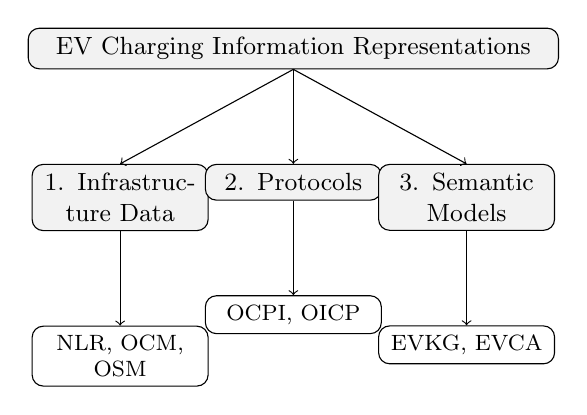
\begin{tikzpicture}[
  node distance=1.2cm and 0.5cm,
  main/.style={rectangle, draw, rounded corners, text width=6.5cm, align=center, fill=gray!10, font=\small},
  sub/.style={rectangle, draw, rounded corners, text width=2.0cm, align=center, fill=white, font=\footnotesize}
]
  \node[main] (root) {EV Charging Information Representations};
  
  \node[main, below=of root, xshift=-2.2cm, text width=2.0cm] (cat1) {1. Infrastructure Data};
  \node[main, below=of root, xshift=0cm, text width=2.0cm] (cat2) {2. Protocols};
  \node[main, below=of root, xshift=2.2cm, text width=2.0cm] (cat3) {3. Semantic Models};
  
  \draw[->] (root.south) -- (cat1.north);
  \draw[->] (root.south) -- (cat2.north);
  \draw[->] (root.south) -- (cat3.north);

  \node[sub, below=of cat1, text width=2.0cm] (sub1) {NLR, OCM, OSM};
  \node[sub, below=of cat2, text width=2.0cm] (sub2) {OCPI, OICP};
  \node[sub, below=of cat3, text width=2.0cm] (sub3) {EVKG, EVCA};

  \draw[->] (cat1.south) -- (sub1.north);
  \draw[->] (cat2.south) -- (sub2.north);
  \draw[->] (cat3.south) -- (sub3.north);
\end{tikzpicture}
\caption{Hierarchy of existing EV charging information representations}
\label{fig:hierarchy}
\end{figure}

\section{Comparative Analysis}
comparative analysis

\begin{table}[t!]
  \centering
  \caption{Comparison of existing EV charging data models.}
  \label{tab:comparison}
  \vspace{-1em}
  \scriptsize
  \setlength{\tabcolsep}{3pt}
  \renewcommand{\arraystretch}{1.1}
  \begin{tabularx}{\columnwidth}{@{}l
      >{\raggedright\arraybackslash}X
      >{\raggedright\arraybackslash}X
      >{\raggedright\arraybackslash}X@{}}
    \toprule
    \textbf{Model} & \textbf{Key entities} & \textbf{Strengths} & \textbf{Limitations} \\
    \midrule
    NLR & Station (flat record) & National, open; coded access and vehicle class & Hours as free text; one network field \\
    OCM & POI, Connection, Operator & Per-connector type, power, quantity & Hours in free text; 83\% from the U.S. Department of Energy dataset; 19\% no operator \\
    OSM & Tagged node & Keys for owner, operator, network, hours & Keys rarely filled (owner 0\%) \\
    OCPI & Location, EVSE, Connector & Structured hours, parking, roles & Not public (B2B only) \\
    EVKG & Station, Network, ConnectorType & Vehicle--connector matching & Hours as string; no adapters or membership \\
    EVCA & Station, Neighbourhood, Trip & Links charging to mobility data & No hours or access; operator only \\
    \bottomrule
  \end{tabularx}
  \vspace{-1.5em}
\end{table}

\section{Entity-Relationship Diagram and Project Positioning}

\bibliographystyle{ACM-Reference-Format}
\bibliography{bibliography.bib}
%\newpage
% \begin{figure*}
%     \centering
% \includegraphics[]{figures/
% .pdf}
%   \caption{The draft version of our project's ER diagram.}
% \end{figure*}
\end{document}
